
% !TEX root = NotesDeCours.tex



\part{Ecoulements compressibles}

% ================================================================================================ 
% Page de titre :
% ================================================================================================

\begin{frame}

  \color{bleu}

  \begin{flushleft}
    
    \Large
   	\bf
    
    Mécanique des fluides 
    
  \end{flushleft}
  
  \ligne{3} % remplace: \noindent \thickline{0.5mm}{150}

  \begin{flushright}

    \rm

    \textrm{David} \textsc{Fabre}
    
    \vspace{3mm}
    
    IMFT / UPS
    
    Département de Mécanique
    


  \end{flushright}


\begin{picture}(110, 35)(0, 1)
  \put(0,  0){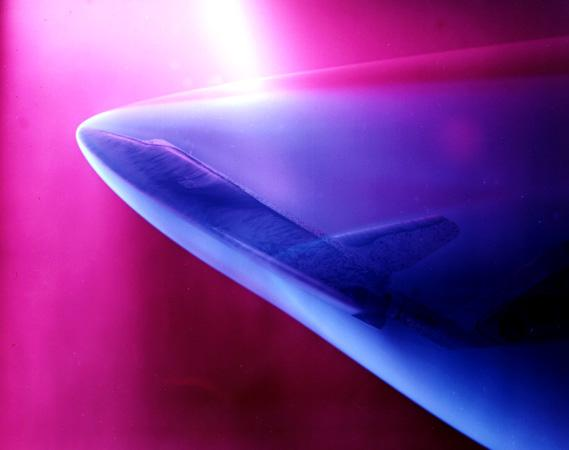
\includegraphics[height=50mm]{shock_wave_wind_tunnel.jpg}}
  %\put(36,  0){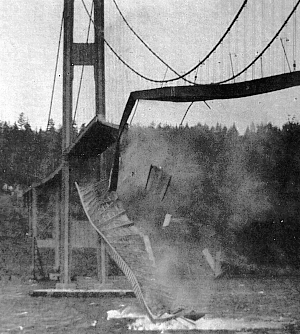
\includegraphics[height=40mm]{tacoma02_crop.png}}
  \put(66, 8){\color{gris} \small \rm 
  \begin{minipage}{34mm}
  									Onde de choc à l'avant \\
									de la Navette Spatiale \\
									lors de la rentrée dans \\ l'atmosphère.\\
									Expérience en soufflerie \\ supersonique.
	\end{minipage}}
\end{picture}

  \vspace{5mm}
  
  \begin{flushright}
    
    \Large
   	\bf
    
    12. Ondes de choc

  \end{flushright}

  \vspace{5mm}

\end{frame}

%\end{document}

%%%%%%%%%%%%%%%%%%%%%%%%%%%%%%%%%%%%%%%%%%%%%%%%%%%%%%%%%%%%%%%%%%%%%%%%%%%%%%%%%%%%%%%%%%
% Sommaire :
%%%%%%%%%%%%%%%%%%%%%%%%%%%%%%%%%%%%%%%%%%%%%%%%%%%%%%%%%%%%%%%%%%%%%%%%%%%%%%%%%%%%%%%%%%

\begin{frame}{Sommaire}

\small
  
\hspace*{2mm}
\begin{tabular}{cc}
		%&
  		\begin{minipage}{62mm}
  			\tableofcontents[firstsection=-10]
      \vspace{15mm}
  		\end{minipage}
  		&   
  		\begin{minipage}{60cm}
		  \vspace*{-5mm}  
  			%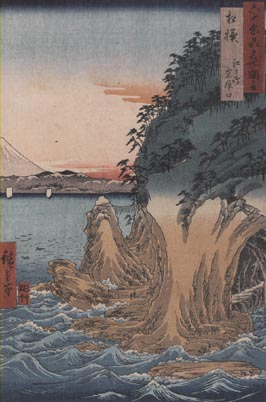
\includegraphics[width=40mm]{vagues.jpg} 
  		\end{minipage}
  	\end{tabular}

\vspace{0mm}

\end{frame}

%%%%%%%%%%%%%%%%%%%%%%%%%%%%%%%%%%%%%%%%%%%%%%%%%%%%%%%%%%%%%%%%%%%%%%%%%%%%%%%%%%%%%%%%%%
\section{\bfseries Ondes de choc}
%%%%%%%%%%%%%%%%%%%%%%%%%%%%%%%%%%%%%%%%%%%%%%%%%%%%%%%%%%%%%%%%%%%%%%%%%%%%%%%%%%%%%%%%%%

%==========================================================================================
\subsection{Introduction}
%=========================================================================================

%-----------------------------------------------------------------------------------------
\subsubsection{Contexte et motivations}
%-----------------------------------------------------------------------------------------
\begin{frame}{Contexte et motivations}
%-----------------------------------------------------------------------------------------

\small

\textbf{Cadre des chapitres précédents (10 et 11) :} \medskip

limité aux variations lentes et isentropiques
des grandeurs thermodynamiques $p$, $\rho$, $T$, \ldots \\ 
et de la vitesse $\myvec{u}$

\vspace{3mm}

Mais\ldots \pause

\vspace{3mm}

\textbf{Observations expérimentales :} \medskip

les écoulements compressibles à grande vitesse peuvent subir des variations extrêmement 
brusques de leurs caractéristiques

\smallskip
\hspace{5mm}
{\color{gris} \checkmark \; par ex. décélération des particules fluides de l'ordre de $10^9$ m/s$^2$}

\pause

\smallskip
sur des distances très faibles

\smallskip
\hspace{5mm}
{\color{gris} \checkmark \; 
par ex. de l'ordre de $10^{-7}$ m = 0.1 $\mu$m $\sim$ libre parcours moyen de molécules de gaz}

\vspace{7mm}

\begin{center}
	\color{vert} $\rightarrow$  \; Notion de choc
\end{center}

\vspace{5mm}

\end{frame}

%-----------------------------------------------------------------------------------------
\subsubsection{Phénoménologie -- Observations}
%-----------------------------------------------------------------------------------------
\begin{frame}{Ondes acoustiques, effet Doppler et mur du son}
%-----------------------------------------------------------------------------------------

\small

Déplacement à vitesse $u$ d'un corps dans l'air 
$\rightarrow$ génération d'ondes de pression de célérité $c$


\begin{picture}(100, 43)(0, 0)
	\put(7, 35){$u \ll c$}
	\put(5, 32){$(M \ll 1)$}
	\put(0, 3){\animategraphics[height=25mm]{10}{Figures/Doppler/doppler1-}{0}{49}}
	\put(1.5, 0){quasi-incompressible}
%	\pause
	\put(33, 35){$u < c$}
	\put(31, 32){$(M < 1)$}
	\put(26, 3){\animategraphics[height=25mm]{10}{Figures/Doppler/doppler2-}{0}{49}}
	\put(32, 0){subsonique}
%	\pause

	\put(59, 35){$u = c$}
	\put(57, 32){$(M = 1)$}
	\put(52, 3){\animategraphics[height=25mm]{10}{Figures/Doppler/doppler4-}{0}{49}}
	\put(59, 0){sonique}
%	\pause
	\put(87, 35){$u > c$}
	\put(85, 32){$(M > 1)$}
	\put(80, 3){\animategraphics[height=25mm]{10}{Figures/Doppler/doppler5-}{0}{49}}
	\put(85, 0){supersonique}
\end{picture}

\vspace{2mm}

{\hyperlink{frame:effet_doppler}{\hspace*{29mm} [effet Doppler]}}


\vspace{0mm}

\end{frame}

%-----------------------------------------------------------------------------------------
\begin{frame}{Ondes de choc : vol supersonique}
%-----------------------------------------------------------------------------------------

\small

\begin{picture}(100, 60)(-2, 0)
	\put(0, 4){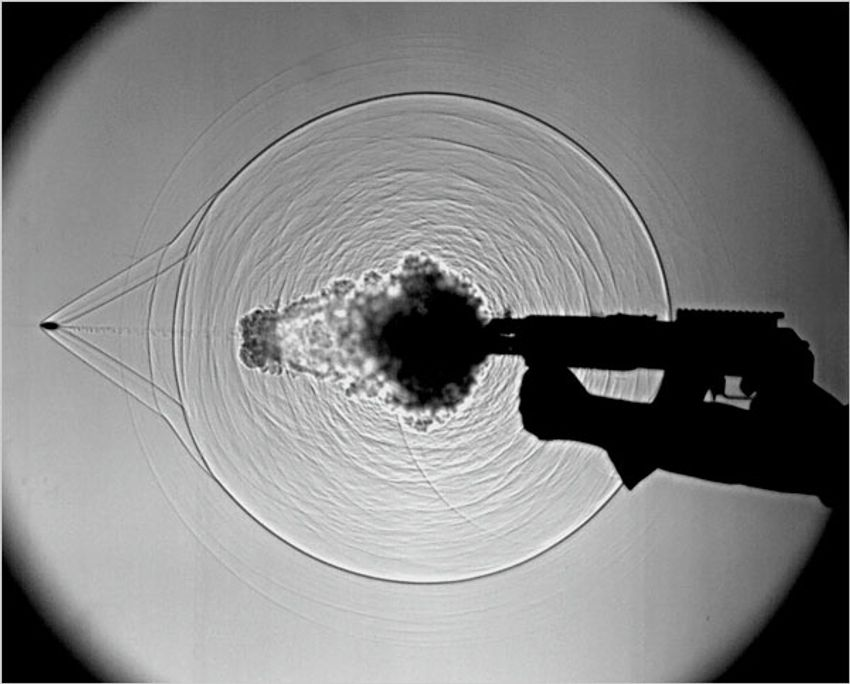
\includegraphics[height=45mm]{AK47_shock_wave.jpg}}
	\put(2, 0){Tir de fusil d'assaut (AK-47)}
\pause
    \put(57, 18.85){\movie[height=30mm,poster,externalviewer,showcontrols=false]%
    								 			{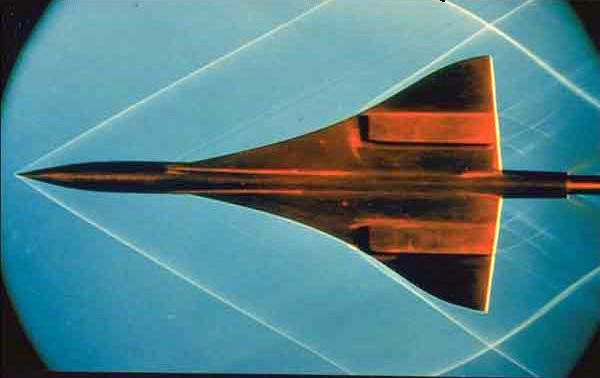
\includegraphics[height=30mm]{Concorde.jpg}}%
								   			{./Figures/F14_shockwave.mpeg}}
	\put(78, 15){Maquette du Concorde}
	\put(75, 12){en soufflerie supersonique}
\end{picture}

\vspace{25mm}

\end{frame}

%-----------------------------------------------------------------------------------------
\begin{frame}{Ondes de choc : Super-Sonic Car (SSC)}
%-----------------------------------------------------------------------------------------

\small

\begin{picture}(110, 65)(-5, 0)
	\put(0, 34){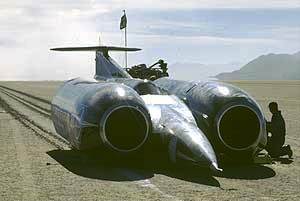
\includegraphics[height=32mm]{SSC_photo.jpg}}
	\put(50, 34){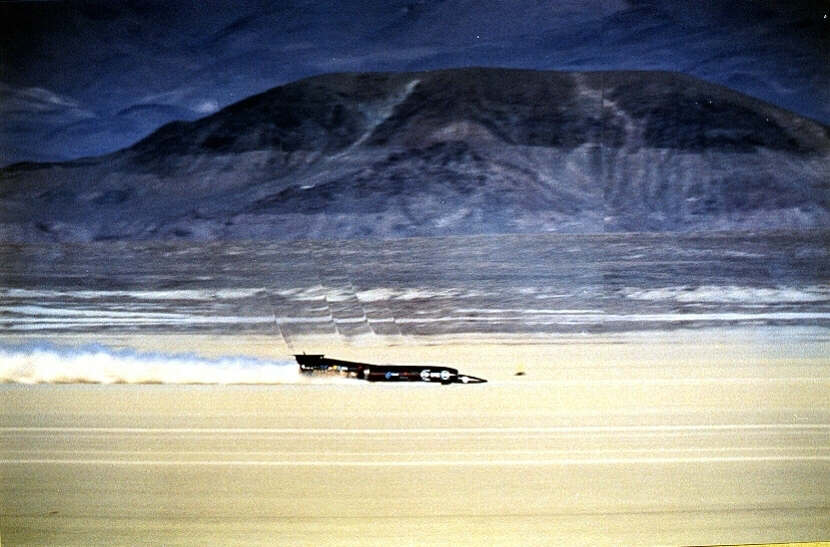
\includegraphics[height=32mm]{SSC_shockwaves.jpg}}
	\put(0, 0){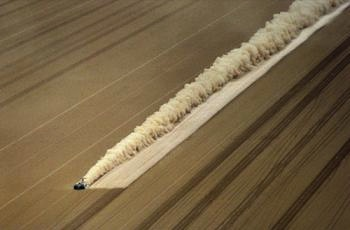
\includegraphics[height=31.5mm]{SSC_front_shockwave.jpg}}
	\put(50, 0){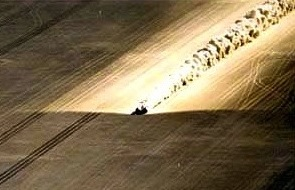
\includegraphics[height=31.5mm]{SSC_shockwave_zoom.jpg}}
\end{picture}


\vspace{0mm}

\end{frame}

%-----------------------------------------------------------------------------------------
\begin{frame}{Ondes de choc : explosions}
%-----------------------------------------------------------------------------------------

\small

\begin{picture}(100, 45)(-2, 0)
	\put(0, 10){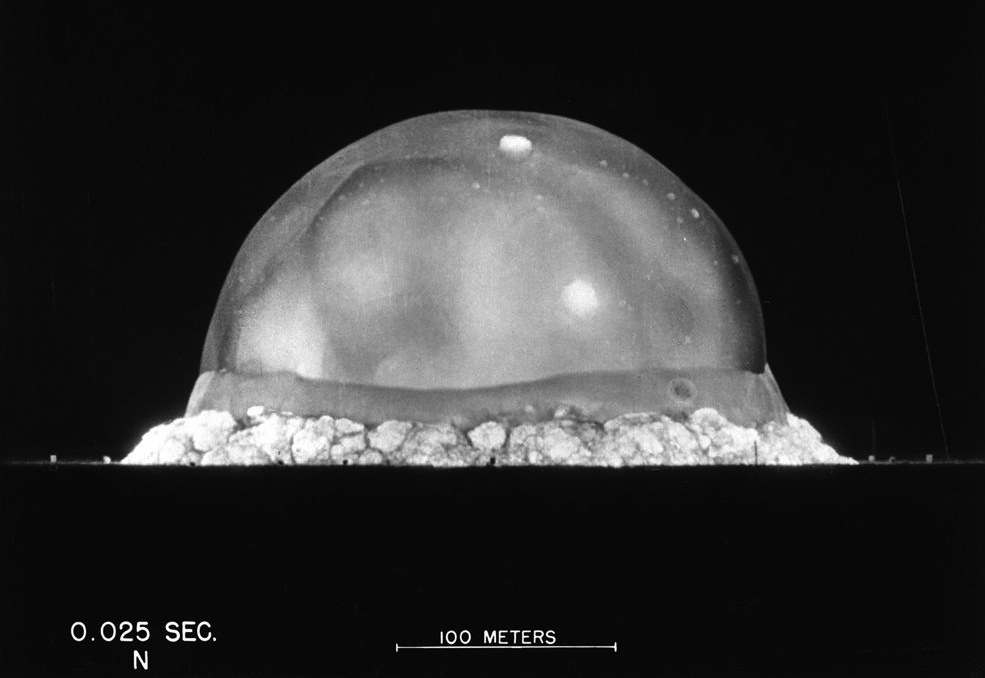
\includegraphics[height=35mm]{Trinity2.jpeg}}
	\put(52, 10){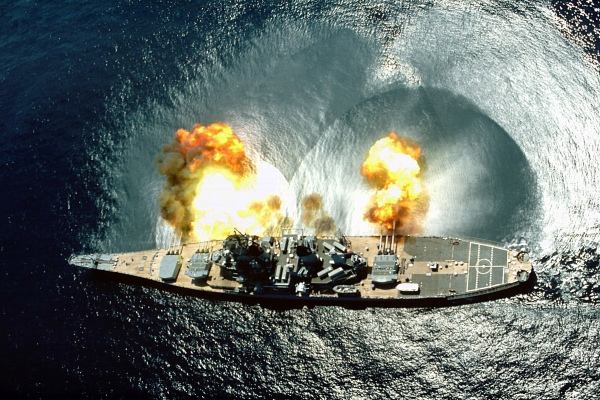
\includegraphics[height=35mm]{USS_Iowa_BB61.jpg}}
	\put(1, 0){\begin{minipage}{49mm}
							\tt The expanding fireball and shockwave of the Trinity explosion, 
							seen .025 seconds after detonation on July 16, 1945. 
							(U.S. Department of Defense)
						  \end{minipage}}
	\put(54.5, -5.35){\begin{minipage}{49mm}
							\tt The USS Iowa is firing shells from its cannon that travel 
							about twice the speed of sound. 
							While the shells themselves will likely produce their own shock waves 
							as they travel through the air, it is the shock wave caused 
							by the explosion of the cannons that is visible on the water.
						  \end{minipage}}
\end{picture}


\vspace{15mm}

\end{frame}

%-----------------------------------------------------------------------------------------
\begin{frame}{Onde de choc dans les liquides : coup de bélier}
%-----------------------------------------------------------------------------------------

\small

\begin{picture}(110, 67)(-5, 0)
	\put(0, 31){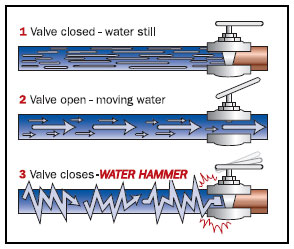
\includegraphics[height=36mm]{coup_belier_dessin.jpg}}
	\put(49.9, 32){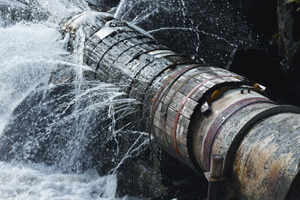
\includegraphics[height=34mm]{coup_belier1.jpg}}
	\put(1, 0){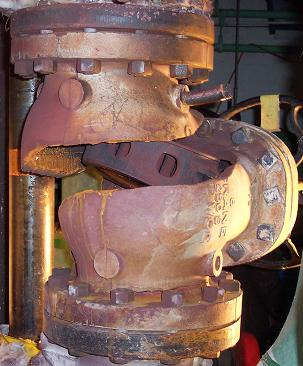
\includegraphics[height=30mm]{coup_belier4.jpg}}
	\put(26.8, 0){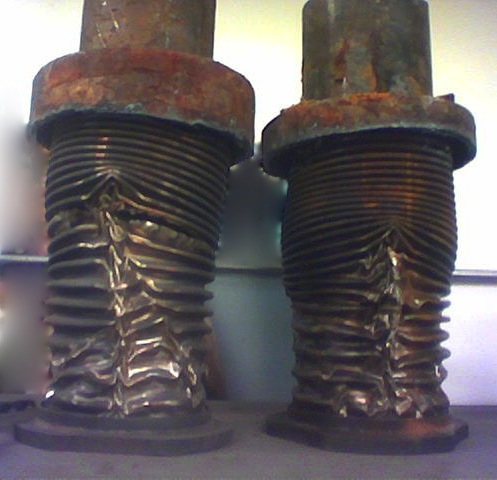
\includegraphics[height=30mm]{coup_belier2.jpg}}
	\put(59, 0){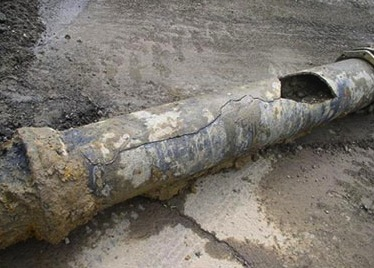
\includegraphics[height=30mm]{coup_belier3.jpg}}
\end{picture}


\vspace{0mm}

\end{frame}

%-----------------------------------------------------------------------------------------
\begin{frame}{Régime discontinu d'une tuyère amorcée}
%-----------------------------------------------------------------------------------------

\small

\begin{picture}(120, 63)
	\put(2, 35){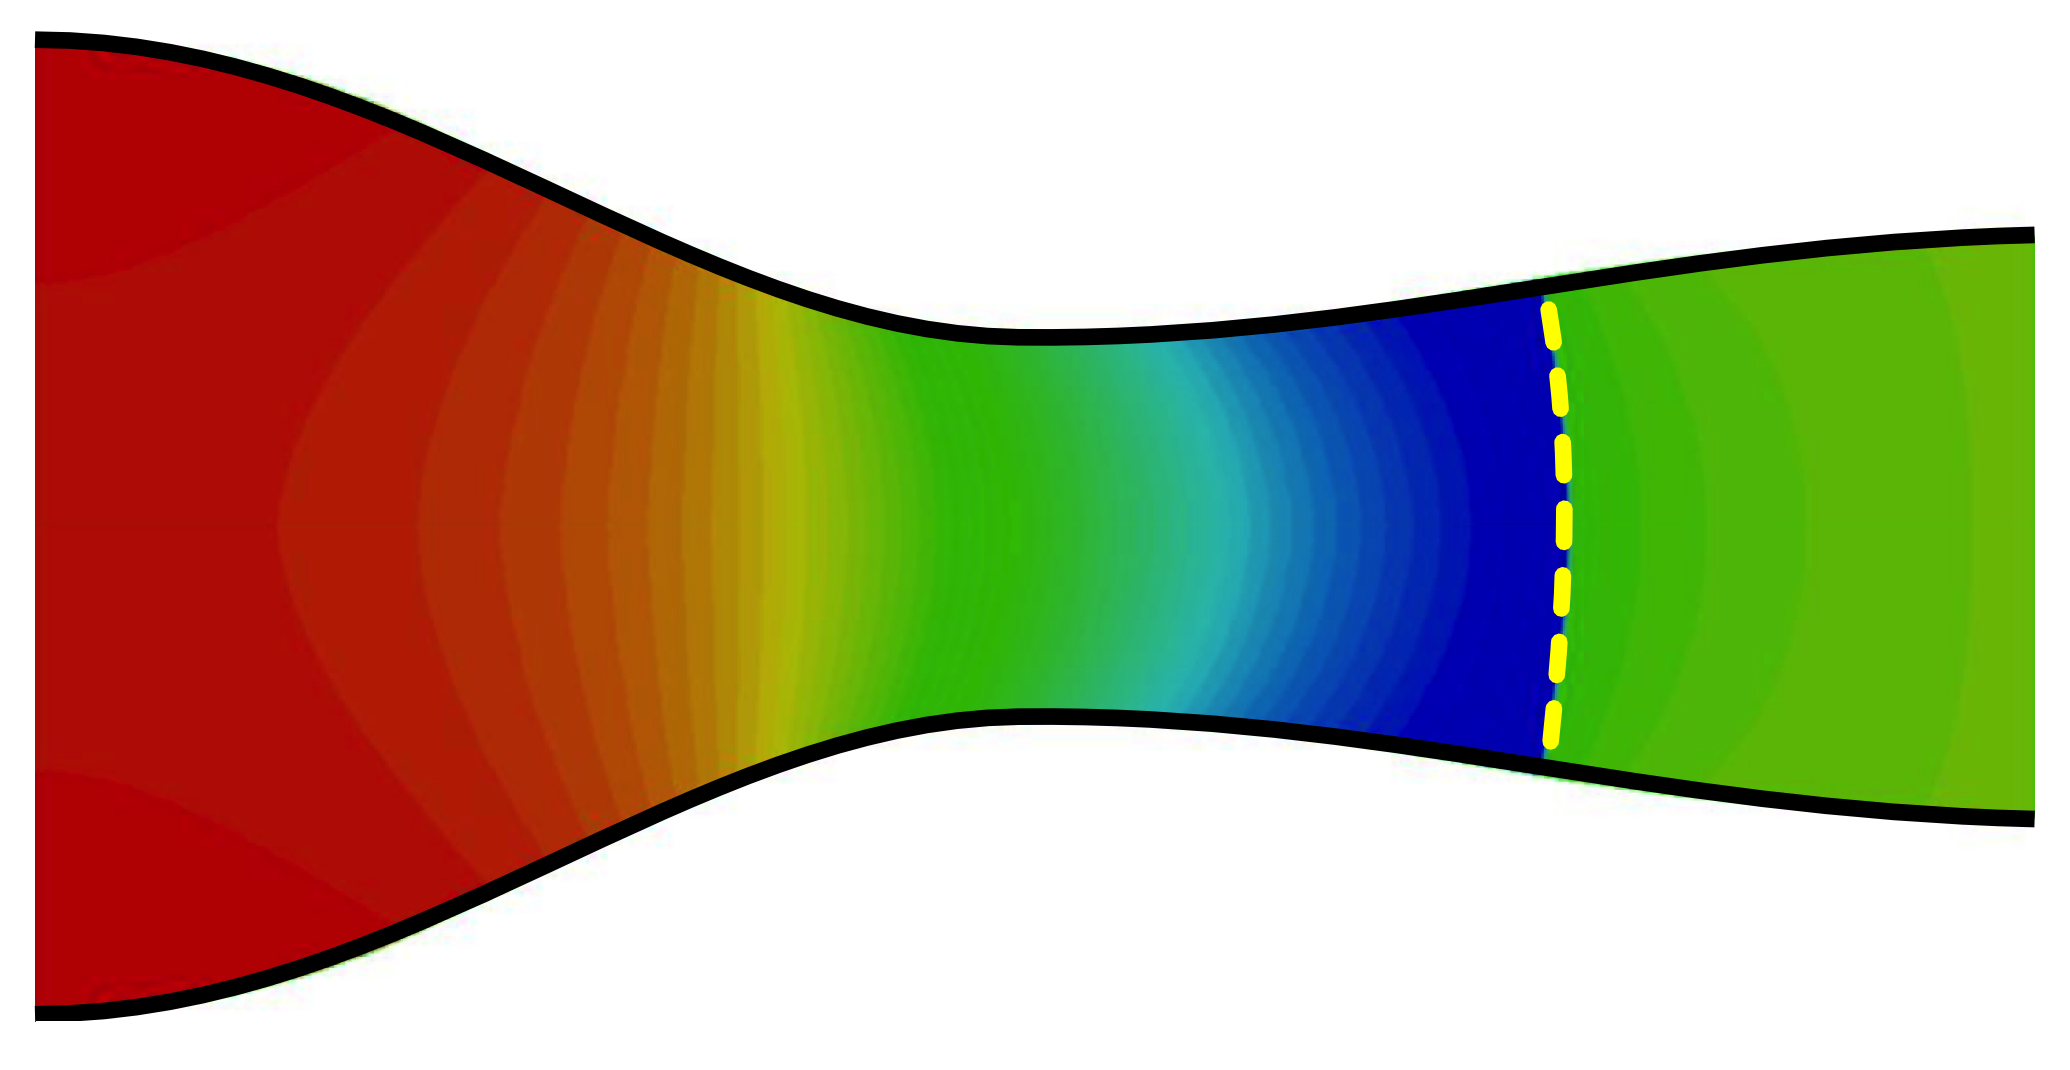
\includegraphics[width=50mm]{Nozzle/pressurein_nozzle.png}}
	\put(55, 40){
\includegraphics[height=16mm, width=3mm]{Nozzle/colorbar.png}}
	\put(0, 18){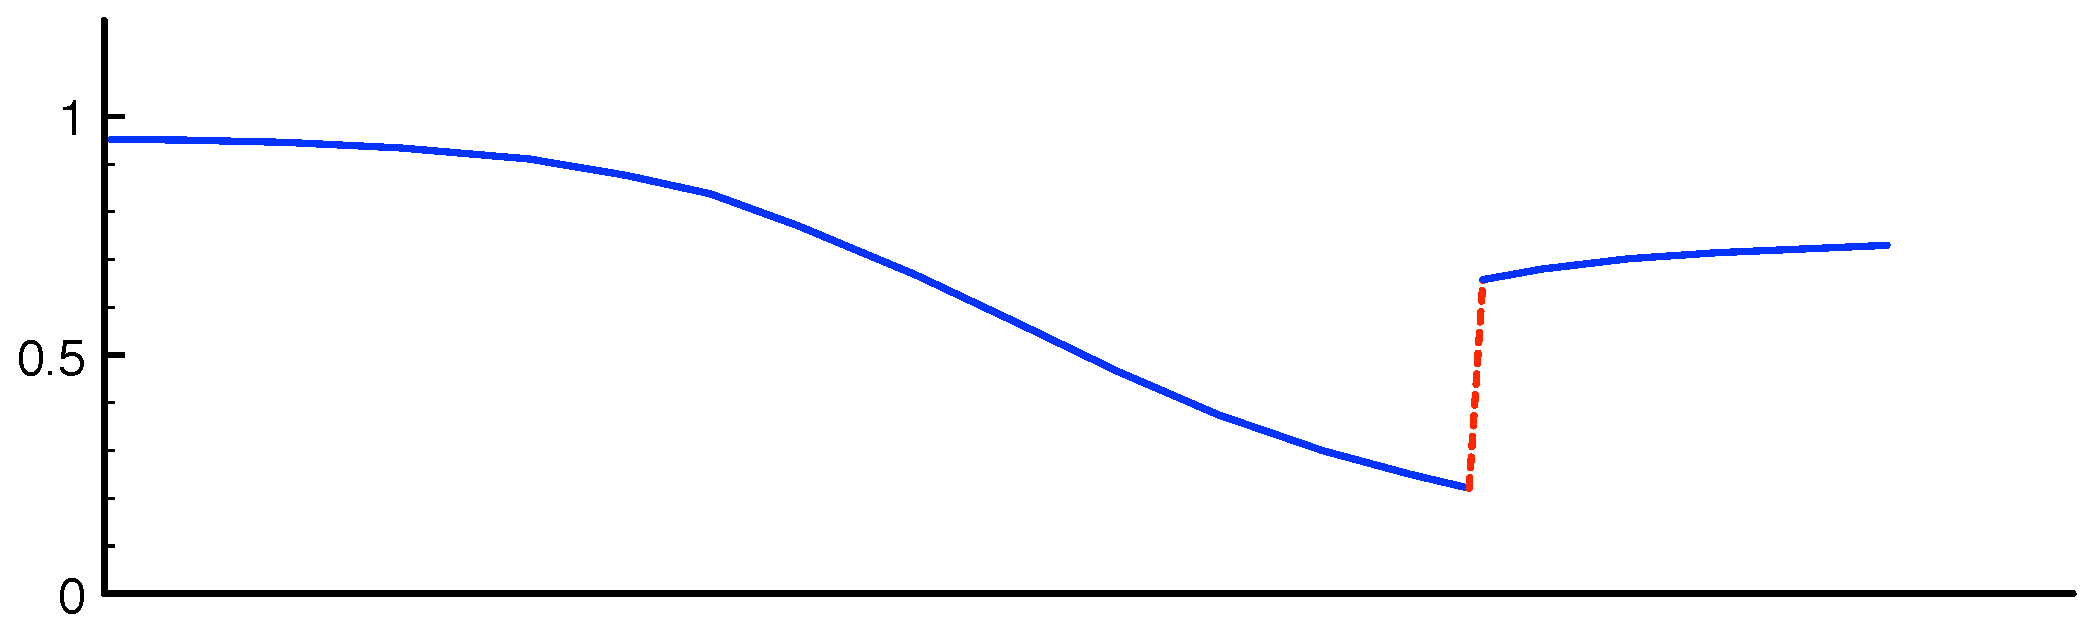
\includegraphics[width=55mm]{Nozzle/pressure.pdf}}
	\put(0, 0){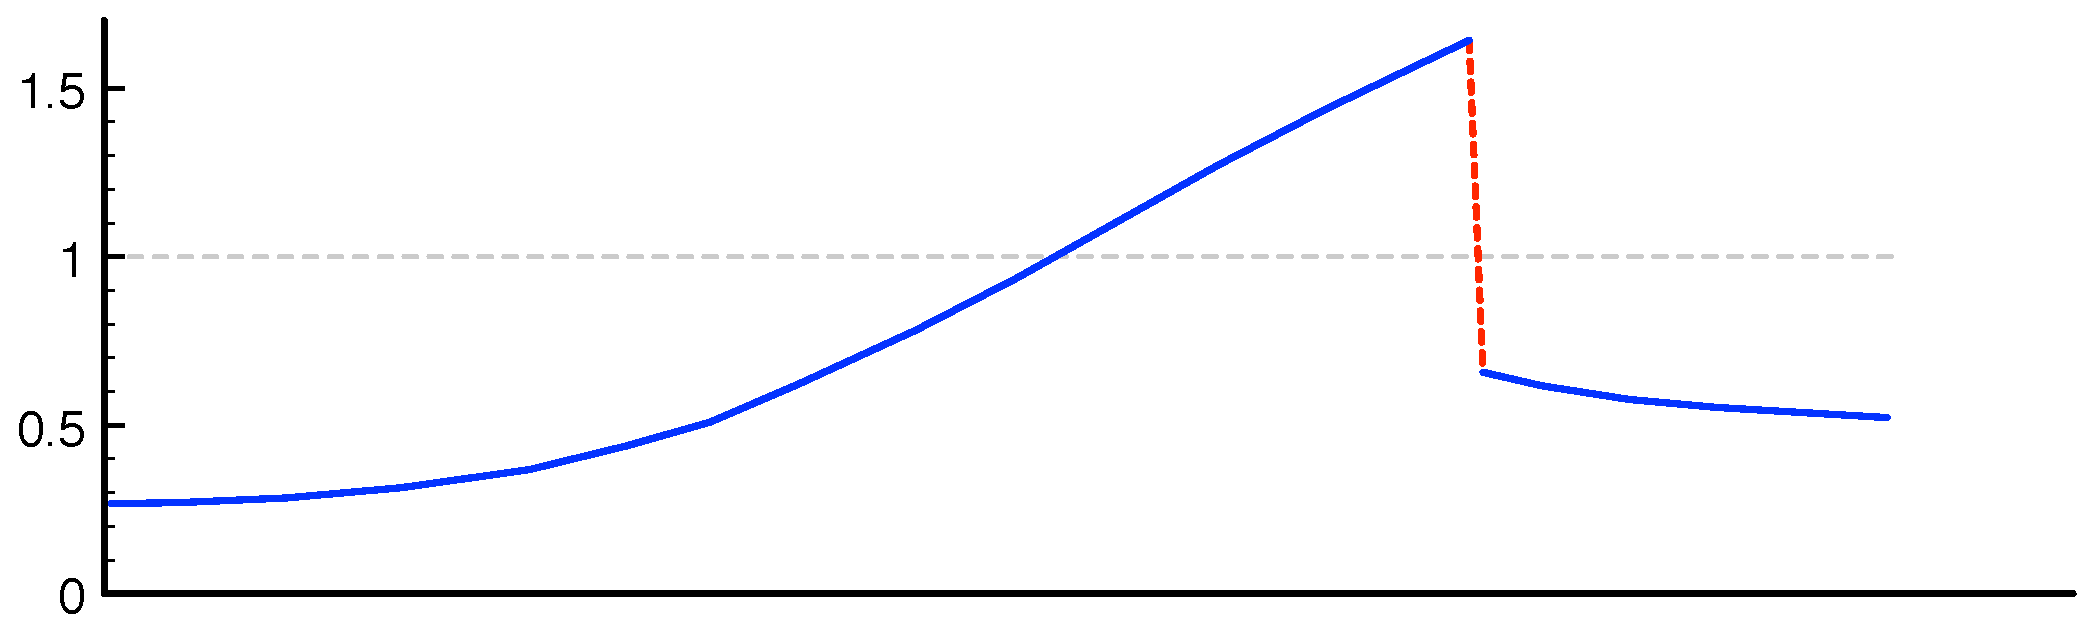
\includegraphics[width=55mm]{Nozzle/Mach_nozzle.pdf}}
	\put(27.7, 0){\color{vert}\line(0, 1){54}}
	\put(4, 48.2){\color{yellow}\vector(1, 0){5}}
	\put(25, 38){\colorbox{white}{\color{vert}col}}
	\put(54, 58){$p/p_i$}
	\put(10, 61){champ de pression dans la tuyère}
	\put(15, 58){(simulation Fluent \copyright)}
	\put(4, 25){$p/p_i$}
	\put(4, 7){$M$}
	\put(39.2, 36.5){\color{rouge} \vector(0, 1){5}}
	\put(39.2, 32.7){\color{rouge} \vector(0, -1){5}}
	\put(52.2, 32.2){\color{vert} $p_{\mbox{\scriptsize ext}}/p_i$}
	\put(55.2, 28.1){\color{vert} \line(0, 1){3}}
	\put(55.2, 28.1){\color{vert} \vector(-1, 0){5}}
	\put(36, 34){\color{rouge} \bf CHOC}
	\put(66, 32){\begin{minipage}{40mm}
									Si la pression en sortie de tuyère 
									n'est pas adaptée à la pression extérieure
									
									\medskip
							 		$\rightarrow$ existence d'un choc d'adaptation 
									\mytabbing{$\rightarrow$} dans le divergent 
									
									\medskip
									$\rightarrow$ après le choc, l'écoulement 
									\mytabbing{$\rightarrow$} redevient subsonique et décélère
									\mytabbing{$\rightarrow$} (cf. relation d'Hugoniot)
									
									\bigskip
									
									Ce régime de fonctionnement est donc à éviter puisqu'il ne permet 
									pas d'accélérer continûment l'écoulement jusqu'en sortie de tuyère.
									
									\bigskip
									Il n'est alors pas possible d'obtenir une poussée optimale.
					    \end{minipage}}
\end{picture}


\vspace{0mm}

\end{frame}

%==========================================================================================
\subsection{Equations de bilan à travers un choc droit}
%=========================================================================================

%-----------------------------------------------------------------------------------------
\subsubsection{Modélisation}
%-----------------------------------------------------------------------------------------
\begin{frame}{Modélisation}
%-----------------------------------------------------------------------------------------

\small

\textbf{Principe :} \medskip

On s'intéresse aux variations des grandeurs physiques à travers l'onde de choc :

\medskip

$\rightarrow$ 
on peut ignorer la structure détaillée de l'onde de choc qui sera alors considérée 
\mytabbing{$\rightarrow$} 
comme une \textcolor{vert}{surface de discontinuité} des grandeurs physiques
$u$, $\rho$, $p$, $T$, \ldots

\bigskip \pause

On se restreint au cas du choc droit : plan et perpendiculaire à l'écoulement 

\smallskip
\hfill {\color{gris}$\rightarrow$ choc oblique ou courbe : cf. master}

\bigskip 

\pause

\textbf{Hypothèses :}

\begin{itemize}
\item
choc droit stationnaire fixe, adiabatique
\item
gaz parfait (non conducteur de la chaleur, non visqueux)
\item
écoulement stationnaire
\item
forces de volume négligeables
\item
pas de réaction chimique
\end{itemize}

\vspace{5mm}

\end{frame}

%-----------------------------------------------------------------------------------------
\subsubsection{Application des principes de conservation}
%-----------------------------------------------------------------------------------------
\begin{frame}{Volume de contrôle}
%-----------------------------------------------------------------------------------------

\small

Soit le volume de contrôle fixe infinitésimal $\Omega$, de normale sortante $\myvec{n}$,
suivant :

\begin{center}
	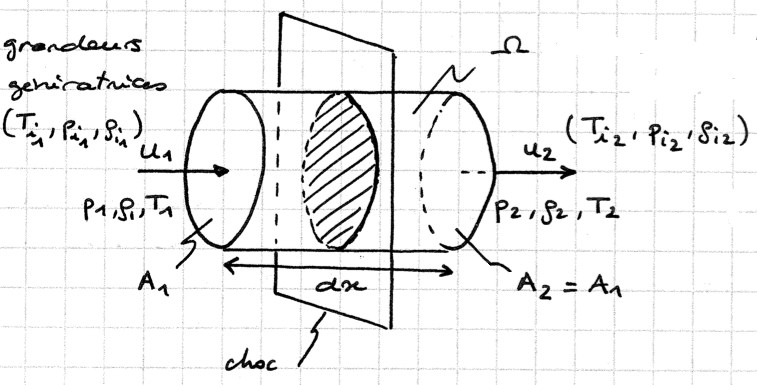
\includegraphics[width=80mm]{volume_controle_choc.png}
\end{center}

On notera par l'indice 1 toute quantité physique \textsl{juste avant le choc} (amont), et
\mytabbing{On notera} par l'indice 2 toute quantité physique \textsl{juste après le choc} (aval).

\vspace{5mm}

\end{frame}

%-----------------------------------------------------------------------------------------
\begin{frame}{Bilans de masse et de quantité de mouvement}
%-----------------------------------------------------------------------------------------

\small

\begin{picture}(0, 0)(0, 25)
	\put(65, 0){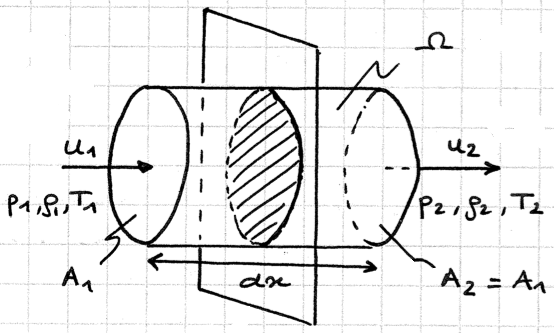
\includegraphics[width=50mm]{volume_controle_small.png}}
\end{picture}

\begin{minipage}{55mm}
Bilan intégral de masse :
\[
	\color{bleu}
	\dpdt{} \int_\Omega \rho \, dV = - \oint_{\partial \Omega} \rho \myvec{u} \cdot \myvec{n} \, dS
\]
\pause
\[
\Rightarrow \quad 0 = \rho_1 u_1 A_1 - \rho_2 u_2 A_2
\] 
\pause
D'où
\begin{equation}
	\color{rouge}
	\rho_1 u_1 = \rho_2 u_2
\end{equation}

\end{minipage}

\vspace{5mm}

\pause

Bilan intégral de quantité de mouvement :
\[
	\color{bleu}
	\dpdt{} \int_\Omega \rho \myvec{u} \, dV 
	= 
	- \oint_{\partial \Omega} \rho \myvec{u} (\myvec{u} \cdot \myvec{n}) \, dS
	- \oint_{\partial \Omega} p\myvec{n} \, dS
\]
\pause
\[
\Rightarrow \quad 0 = \rho_1 u_1^2 A_1 - \rho_2 u_2^2 A_2 + p_1 A_1 - p_2 A_2
\] 
\pause
D'où
\begin{equation}
	\color{rouge}
	p_1 + \rho_1 u_1^2 = p_2+\rho_2 u_2^2
\end{equation}

\vspace{5mm}

\end{frame}

%-----------------------------------------------------------------------------------------
\begin{frame}{Bilan d'énergie}
%-----------------------------------------------------------------------------------------

\small

\begin{picture}(0, 0)(0, 30)
	\put(65, 0){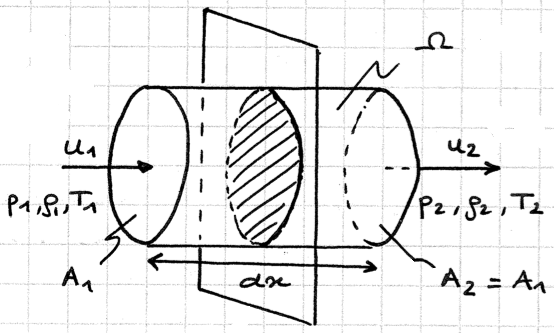
\includegraphics[width=50mm]{volume_controle_small.png}}
\end{picture}

\begin{minipage}{65mm}
Bilan intégral d'énergie :

\medskip

$\displaystyle
	\color{bleu}
	\dpdt{} \int_\Omega \rho \left ( e+\frac{1}{2} u^2 \right ) \, dV
$
\medskip

\hspace{5mm} {\color{bleu}$=$} 
$\displaystyle 
  \color{bleu} - \oint_{\partial \Omega} \rho \left ( e+\frac{1}{2} u^2 \right ) \myvec{u} \cdot \myvec{n} \, dS
$

\medskip

\hspace{5mm} {\color{white}$=$} 
$\displaystyle
	\color{bleu} + \, \mathcal{P}_{m, ext}
	+ \mathcal{P}_{th, ext}
$

\medskip \pause

\hspace{1mm} $\Rightarrow$
$\displaystyle
	\oint_{\partial \Omega} \rho \left ( e+\frac{1}{2} u^2 + \frac{p}{\rho}\right ) \myvec{u} \cdot \myvec{n} \, dS = 0
$
\; (chap. 11)

\end{minipage}

\pause

\smallskip

\[
\Rightarrow \quad \rho_1 u_1 A_1 \left ( e_1+\frac{1}{2} u_1^2 + \frac{p_1}{\rho_1}\right ) 
- \rho_2 u_2 A_2 \left ( e_2+\frac{1}{2} u_2^2 + \frac{p_2}{\rho_2}\right ) = 0
\] 

\pause

\smallskip

Or $\rho_1 u_1 = \rho_2 u_2$ et $A_1 = A_2$ 
$ \displaystyle
\quad \Rightarrow \quad	e_1+\frac{1}{2} u_1^2 + \frac{p_1}{\rho_1} = e_2+\frac{1}{2} u_2^2 + \frac{p_2}{\rho_2}
$
\pause
\smallskip

avec enthalpie spécifique $h = e+p/\rho = C_p T$ :

\begin{equation}
	\color{rouge}
	C_p T_1 + \frac{u_1^2}{2} = C_p T_2 + \frac{u_2^2}{2}
\end{equation}

\pause
Remarque : enthalpie totale $H = h +u^2/2$ $\, \Rightarrow \, H_1 = H_2$ 
\mytabbing{Remarque :} donc \textcolor{rouge}{l'enthalpie totale est conservée à la traversée du choc !}

\vspace{5mm}

\end{frame}

%-----------------------------------------------------------------------------------------
\begin{frame}{Bilan d'entropie}
%-----------------------------------------------------------------------------------------

\small

\begin{picture}(0, 0)(0, 25)
	\put(65, 0){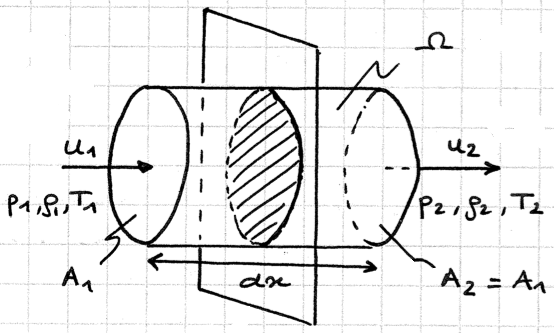
\includegraphics[width=50mm]{volume_controle_small.png}}
\end{picture}

\begin{minipage}{50mm}

Choc = siège de phénomènes irréversibles \\ (visqueux et thermiques)

\bigskip

Le second principe impose donc :

\begin{equation}
	\color{rouge}
	s_2 > s_1
\end{equation}

\end{minipage}

\vspace{40mm}

\end{frame}

%==========================================================================================
\subsection{Relations de saut à travers le choc droit}
%=========================================================================================

%-----------------------------------------------------------------------------------------
\subsubsection{Rapports aval/amont}
%-----------------------------------------------------------------------------------------
\begin{frame}{Rapports aval/amont (1)}
%-----------------------------------------------------------------------------------------

\small

\textbf{Objectif :} 
déterminer $\dfrac{u_2}{u_1}(M_1)$, $\dfrac{\rho_2}{\rho_1}(M_1)$, 
$\dfrac{p_2}{p_1}(M_1)$, $\dfrac{T_2}{T_1}(M_1)$

\bigskip

\pause

$\rightarrow$ Equation pour l'énergie (3) : 

\[ \color{bleu}
	C_p T_1 + \dfrac{u_1^2}{2} = C_p T_2 + \dfrac{u_2^2}{2}
\]
\pause
avec
\[
C_p T + \dfrac{u^2}{2} = C_p T \left ( 1 + \dfrac{u^2}{2C_p T} \right )
= C_p T \left ( 1 + \dfrac{\gamma - 1}{2}\dfrac{u^2}{\gamma r T} \right )
= C_p T \left ( 1 + \dfrac{\gamma - 1}{2} M^2 \right )
\]

car $\gamma r T = c^2$ et $C_p = \gamma r / (\gamma-1)$\pause, 
d'où :
\[
	C_p T_1 \left ( 1 + \dfrac{\gamma - 1}{2} M_1^2 \right ) = C_p T_2 \left ( 1 + \dfrac{\gamma - 1}{2} M_2^2 \right )
\]

\pause
\medskip
On en déduit la première relation de saut :

\begin{equation}
	\color{rouge}
	\frac{T_2}{T_1} = \frac{1 + \dfrac{\gamma - 1}{2} M_1^2}{1 + \dfrac{\gamma - 1}{2} M_2^2}
\end{equation}


\vspace{5mm}

\end{frame}

%-----------------------------------------------------------------------------------------
\begin{frame}{Rapports aval/amont (2)}
%-----------------------------------------------------------------------------------------

\small

\textbf{Objectif :} 
déterminer $\dfrac{u_2}{u_1}(M_1)$, $\dfrac{\rho_2}{\rho_1}(M_1)$, 
$\dfrac{p_2}{p_1}(M_1)$, $\dfrac{T_2}{T_1}(M_1)$

\bigskip

\pause

$\rightarrow$ Equation pour la quantité de mouvement (2) : 

\[ \color{bleu}
	p_1 + \rho_1 u_1^2 = p_2 + \rho_2 u_2^2
\]
\pause
avec
\[
p+\rho u^2 = p\left ( 1 + \frac{\rho}{p} u^2 \right )
= p\left ( 1 + \gamma \frac{\rho}{\gamma p} u^2 \right ) = p\left ( 1 + \gamma M^2 \right )
\]

car $\gamma p / \rho = c^2$\pause, 
d'où :
\[
	p_1\left ( 1 + \gamma M_1^2 \right ) = p_2\left ( 1 + \gamma M_2^2 \right )
\]

\pause
\medskip
On en déduit la deuxième relation de saut :

\begin{equation}
	\color{rouge}
	\frac{p_2}{p_1} = \frac{1 + \gamma M_1^2}{1 + \gamma M_2^2}
\end{equation}


\vspace{20mm}

\end{frame}

%-----------------------------------------------------------------------------------------
\begin{frame}{Rapports aval/amont (3)}
%-----------------------------------------------------------------------------------------

\small

\textbf{Objectif :} 
déterminer $\dfrac{u_2}{u_1}(M_1)$, $\dfrac{\rho_2}{\rho_1}(M_1)$, 
$\dfrac{p_2}{p_1}(M_1)$, $\dfrac{T_2}{T_1}(M_1)$

\bigskip

\pause

$\rightarrow$ Equation pour la masse (1) : 

\[ \color{bleu}
	\rho_1 u_1 = \rho_2 u_2
\]
\pause
d'où
\[
\frac{\rho_2}{\rho_1} = \frac{u_1}{u_2} = \frac{M_1c_1}{M_2c_2} = \frac{M_1}{M_2} \sqrt{\frac{T_1}{T_2}}
\]

car $c = \sqrt{\gamma r T}$ \pause: 
on en déduit les troisième et quatrième relations de saut :
\begin{equation}
	\color{rouge}
	\frac{\rho_2}{\rho_1} = \frac{u_1}{u_2} = \frac{M_1}{M_2} 
	\sqrt{\frac{1 + \dfrac{\gamma - 1}{2} M_2^2}{1 + \dfrac{\gamma - 1}{2} M_1^2}}
\end{equation}

\pause
Reste à déterminer $M_2$ en fonction de $M_1$\ldots

\vspace{19mm}

\end{frame}


%-----------------------------------------------------------------------------------------
\begin{frame}{Rapports aval/amont (4)}
%-----------------------------------------------------------------------------------------

\small

\textbf{Objectif :} 
déterminer $\dfrac{u_2}{u_1}(M_1)$, $\dfrac{\rho_2}{\rho_1}(M_1)$, 
$\dfrac{p_2}{p_1}(M_1)$, $\dfrac{T_2}{T_1}(M_1)$

\bigskip

\pause

$\rightarrow$ Equation d'état du gaz parfait :

\[ \color{bleu}
	p = \rho r T \quad 
	\pause
	\Rightarrow \quad \frac{p_2}{p_1} = \frac{\rho_2 r T_2}{\rho_1 r T_1}
	= \left ( \frac{\rho_2}{\rho_1} \right ) \left ( \frac{T_2}{T_1} \right )
\]
\pause
D'où, d'après les relations de saut précédentes :
\[
	\frac{1 + \gamma M_1^2}{1 + \gamma M_2^2} =
	\frac{M_1}{M_2} 
	\sqrt{\frac{1 + \dfrac{\gamma - 1}{2} M_2^2}{1 + \dfrac{\gamma - 1}{2} M_1^2}}
	\times
	\frac{1 + \dfrac{\gamma - 1}{2} M_1^2}{1 + \dfrac{\gamma - 1}{2} M_2^2}
	=
	\frac{M_1}{M_2} 
	\sqrt{\frac{1 + \dfrac{\gamma - 1}{2} M_1^2}{1 + \dfrac{\gamma - 1}{2} M_2^2}}
\]
\pause
En élevant au carré :
\[
	\left (\frac{1 + \gamma M_1^2}{1 + \gamma M_2^2} \right )^2=
	\frac{M_1^2}{M_2^2} 
	\left (\frac{1 + \dfrac{\gamma - 1}{2} M_1^2}{1 + \dfrac{\gamma - 1}{2} M_2^2}\right)
\]
\pause
= simple polynôme du second degré en $X = M_2^2$, avec une racine évidente $X = M_1^2$.

\pause

\medskip
On en déduit :
\begin{equation}
	\color{rouge}
	M_2^2 = \frac{2+(\gamma-1)M_1^2}{2\gamma M_1^2 +1-\gamma}
\end{equation}

\vspace{0mm}

\end{frame}


%-----------------------------------------------------------------------------------------
\begin{frame}{Rapports aval/amont (5)}
%-----------------------------------------------------------------------------------------

\small

\textbf{Objectif :} 
déterminer $\dfrac{u_2}{u_1}(M_1)$, $\dfrac{\rho_2}{\rho_1}(M_1)$, 
$\dfrac{p_2}{p_1}(M_1)$, $\dfrac{T_2}{T_1}(M_1)$

\bigskip

En remplaçant
\begin{equation*}
	M_2^2 = \frac{2+(\gamma-1)M_1^2}{2\gamma M_1^2 +1-\gamma}
\end{equation*}

dans les équations de saut obtenues précédemment, on obtient :

\begin{eqnarray}
	\color{rouge} \frac{T_2}{T_1}(M_1) 
	& 
	\color{rouge} = 
	& 
	\color{rouge} \frac{2 + (\gamma-1)M_1^2}{(\gamma+1)^2M_1^2}\left ( 2\gamma M_1^2 + 1 -\gamma\right )
	\\
	\color{rouge} \frac{p_2}{p_1}(M_1) 
	& 
	\color{rouge} = 
	& 
	\color{rouge} 1 + \frac{2\gamma}{\gamma+1}\left ( M_1^2 - 1\right )
	\\
	\color{rouge} \frac{\rho_2}{\rho_1} (M_1) 
	& 
	\color{rouge} = 
	& 
	\color{rouge} \frac{(\gamma+1) M_1^2}{2+(\gamma-1)M_1^2} \quad = \quad \frac{u_1}{u_2}(M_1)
\end{eqnarray}


\vspace{20mm}

\end{frame}

%-----------------------------------------------------------------------------------------
\subsubsection{Saut des grandeurs génératrices}
%-----------------------------------------------------------------------------------------
\begin{frame}{Saut des grandeurs génératrices (1)}
%-----------------------------------------------------------------------------------------

\small

\textbf{Objectif :} 
déterminer $\dfrac{\rho_{i2}}{\rho_{i1}}(M_1)$, 
$\dfrac{p_{i2}}{p_{i1}}(M_1)$, $\dfrac{T_{i2}}{T_{i1}}(M_1)$

\bigskip

$\rightarrow$ Equation pour l'énergie (3) : 

\[ \color{bleu}
	C_p T_1 + \dfrac{u_1^2}{2} = C_p T_2 + \dfrac{u_2^2}{2}
\]
\pause
avec, de chaque côté du choc,
\[
C_p T + \dfrac{u^2}{2} = C_p T_i
\]
\pause
d'où
\[
	\color{bleu} C_p T_1 + \dfrac{u_1^2}{2} = C_p T_{i1} \pause
	\color{black} = \pause
	\color{rouge}{C_p T_2 + \dfrac{u_2^2}{2} = C_p T_{i2}}
\]	
\pause
On en déduit :
\begin{equation}
	\color{rouge}
	T_{i2} = T_{i1}
\end{equation}

\vspace{20mm}

\end{frame}

%-----------------------------------------------------------------------------------------
\begin{frame}{Saut des grandeurs génératrices (2)}
%-----------------------------------------------------------------------------------------

\small

\textbf{Objectif :} 
déterminer $\dfrac{\rho_{i2}}{\rho_{i1}}(M_1)$, 
$\dfrac{p_{i2}}{p_{i1}}(M_1)$, $\dfrac{T_{i2}}{T_{i1}}(M_1)$

\bigskip

$\rightarrow$ Equation d'état du gaz parfait : 

\[ \color{bleu}
	p = \rho r T 
	\pause
	\quad \Rightarrow \quad 
	\frac{p_{i2}}{p_{i1}} = \frac{\rho_{i2} r T_{i2}}{\rho_{i1} r T_{i1}} = \frac{\rho_{i2}}{\rho_{i1}}
\]
car $T_{i2} = T_{i1}$.

\pause
\medskip

On a par ailleurs :
\[
	\frac{p_{i2}}{p_{i1}} 
	= 
	\frac{p_{i2}}{p_{2}} \times \frac{p_{2}}{p_{1}} \times \frac{p_{1}}{p_{i1}}
\]	
où les rapports $p_2/p_{i2}(M_2)$ et $p_1/p_{i1}(M_1)$ sont donnés par les relations isentropiques de St--Venant du chapitre 11, et $p_2/p_1(M_1)$ correspond à la relation de saut (10) déterminée précédemment.

\pause
\medskip

On en déduit :
\begin{equation}
	\color{rouge}
	\frac{p_{i2}}{p_{i1}} = \frac{\rho_{i2}}{\rho_{i1}} = \left \{
	\frac{(\gamma+1)^{\gamma+1} M_1^{2\gamma}}{(2\gamma M_1^2+1-\gamma)\left [ 2+(\gamma-1)M_1^2\right ]^\gamma}
	\right \}^{\dfrac{1}{\gamma - 1}}
\end{equation}

\vspace{7mm}

\end{frame}

%-----------------------------------------------------------------------------------------
\subsubsection{Saut d'entropie}
%-----------------------------------------------------------------------------------------
\begin{frame}{Saut d'entropie}
%-----------------------------------------------------------------------------------------

\small

Le \textcolor{vert}{second principe} impose $\Delta s = s_2 - s_1 > 0$ à travers l'onde de choc : quelle conséquence ?

\bigskip \pause

\textbf{Rappel :} (cf. chapitre 11)
\[
	de = C_v dT = Tds - pdv = Tds - p d(1/\rho) 
	\quad \Rightarrow \quad
	ds = C_v \left ( \frac{dp}{p} - \gamma \frac{d\rho}{\rho}\right )
\]
\pause
d'où
\[
	s = C_v \ln \left ( p\ \rho^{-\gamma}\right )
\quad
\pause
\mbox{et} 
\quad
	\Delta s = C_v \ln\left [\ \frac{p_2}{p_1} \times \left ( \frac{\rho_1}{\rho_2} \right )^\gamma\ \right ]
\]

\pause
Le second principe s'écrit donc 
\[
	\Delta s (M_1) 
	= 
	C_v \ln\left [\ \frac{p_2}{p_1}(M_1) \times \left ( \frac{\rho_1}{\rho_2}(M_1) \right )^\gamma\ \right ]
	> 0
\]

\pause
L'étude de la fonction $\Delta s (M_1)$ montre que : $\Delta s (M_1)>0 \Leftrightarrow M_1 > 1$,
et on en déduit alors que $M_2 < 1$, d'après la relation (8).

\bigskip \pause

\textbf{Conséquence :} \medskip

\color{rouge}
Le second principe impose donc qu'un choc ne peut exister que si l'écoulement est supersonique ($M_1>1$).
De plus, à travers le choc droit, l'écoulement redevient subsonique ($M_2<1$), \\
avec une augmentation de pression, de masse volumique et de température (cf. relations 9 à 11).
\vspace{5mm}

\end{frame}


%==========================================================================================
%\subsection*{Effet Doppler}
%==========================================================================================

%------------------------------------------------------------------------------------------
\begin{frame}{Effet Doppler} \hypertarget{frame:effet_doppler}{}
%------------------------------------------------------------------------------------------

\small

\checkmark \; Effet Doppler = décalage en fréquence dû au mouvement de la source :

\begin{center}
	\begin{picture}(80, 40)
		\put(0, 0){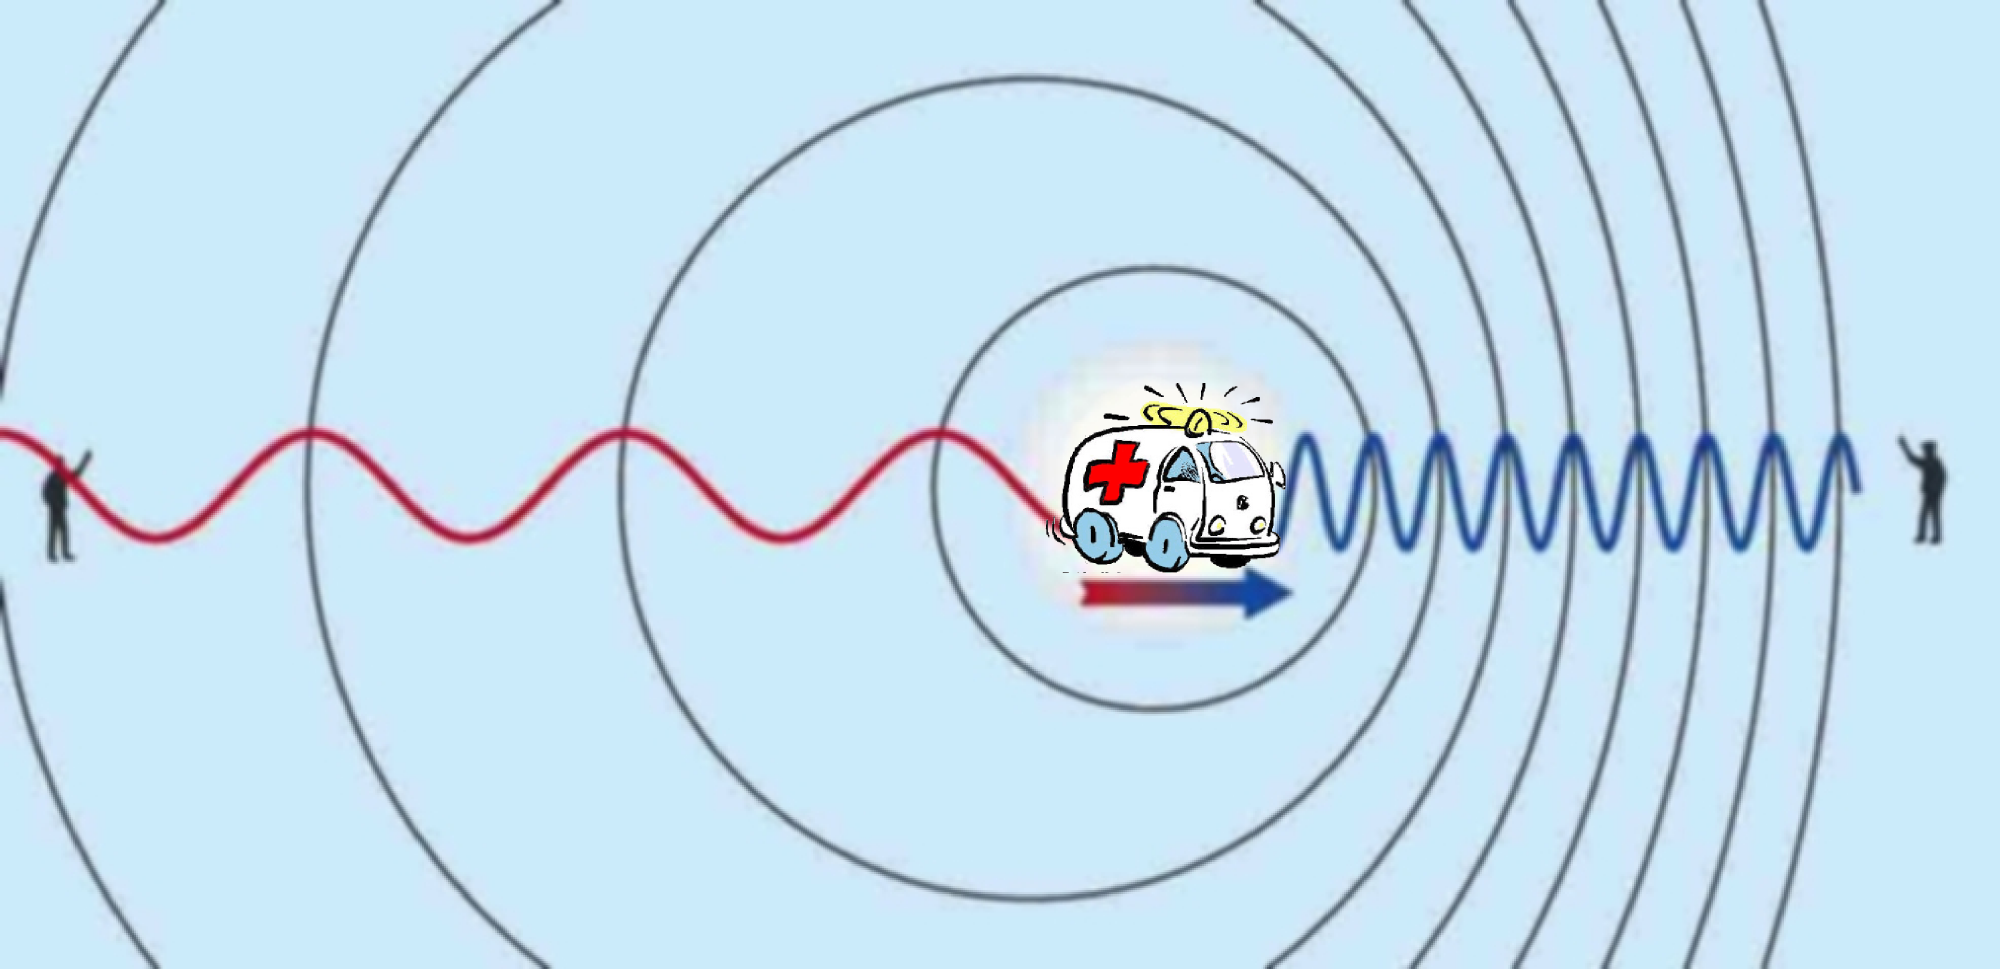
\includegraphics[width=80mm]{Effet_Doppler/effet_doppler.png}}
	\end{picture}
\end{center}

\hspace{10mm}
\begin{minipage}{80mm}
\begin{itemize}
	\item
		\color{bleu}
		véhicule qui approche : longueur d'onde $\lambda$ raccourcie 
		\mytabbing{véhicule qui approche :} $\rightarrow$ haute fréquence $f = c/\lambda$ $\rightarrow$ son aigu
	\item
		\color{rouge}
		véhicule qui s'éloigne : longueur d'onde $\lambda$ rallongée 
		\mytabbing{véhicule qui s'éloigne :} $\rightarrow$ basse fréquence $f = c/\lambda$ $\rightarrow$ son grave
\end{itemize}
\end{minipage}

\vspace{0mm}

\end{frame}


